% Modelo de relatório no estilo artigo em duas colunas
\documentclass[twocolumn]{article}
\usepackage[utf8]{inputenc}
\usepackage{amsmath}
\usepackage{subcaption}
\usepackage{mathtools}
\usepackage{graphicx}
\usepackage{color}
\usepackage{authblk}
\usepackage{lmodern}
% \usepackage[colorlinks,citecolor=black,urlcolor=black,bookmarks=false,hypertexnames=true]{hyperref}
\usepackage[margin=0.9in]{geometry}
\usepackage{pdfpages}
\usepackage{fancyhdr}
\usepackage[utf8]{inputenc}

\usepackage[sorting=none,style=numeric]{biblatex}
\addbibresource{refs.bib}
\usepackage[justification=centering]{caption}
\usepackage{makecell}
\usepackage{booktabs}
\usepackage{hhline}
\usepackage{amsmath}
\usepackage{amssymb}
\usepackage{soul}
\usepackage{gensymb}
\usepackage{listings}

\setlength\parindent{0pt}


\newcommand{\myname}{Nishant Aswani}
\newcommand{\mynetid}{nsa325}
\newcommand{\myemail}{nsa325@nyu.edu}
\newcommand{\myhwtype}{Lab }
\newcommand{\myhwnum}{5}
\newcommand{\mycoursenumber}{ENGR-UH 3511}
\newcommand{\myclassname}{Computer Organization and Architecture}
\newcommand{\myassignmenttitle}{Microprocessor Design and Verilog HDL: Part 3}
\newcommand{\myinstructor}{Cristoforos Vasilatos}

\newcommand{\cc}[1]{\texttt{#1}}

\lstset{
  basicstyle=\ttfamily,
  escapeinside=||
}

% Tamanho das margens:
% \geometry{
% 	a4paper,
% 	total={170mm,257mm},
% 	left=30mm,
% 	top=20mm,
% }
%%%%%%%%%%%%%%%%%%%%%%%%%%%%%%%%%%%%%%%%%
% Bibliografia estilo ABNT. Se não tiver instalado, comente a linha abaixo.
% \usepackage[alf, abnt-etal-list=0, abnt-emphasize=bf,abnt-last-names=bibtex, abnt-etal-text=it, abnt-etal-cite=2]{abntex2cite}
%%%%%%%%%%%%%%%%%%%%%%%%%%%%%%%%%%%%%%%%%

% Dados de identificação
\title{\myassignmenttitle}
\author{\myname, \myemail}
\affil{\myclassname (\mycoursenumber), Instructor \myinstructor}
\date{}

\begin{document}
%%%%%%%%%%%%%%%%%%%%%%%%%%%%%%%%%%%%%%%%%%%%%%%% COVER PAGE %%%%%%%%%%%%%%%%%%%%%%%%%%%%%%%%%%%%%%%%%%%%%%%%%%%%
\onecolumn
\pagestyle{fancy}
\fancyhf{}
\renewcommand{\headrulewidth}{0pt}
\rhead{\textbf{Division of Engineering}}
\lhead{\textbf{NYU Abu Dhabi}}

\begin{center}
  
\includegraphics[scale=0.15]{etc/NYUAD-alt-logo.jpg}
\end{center}

{\vspace{2.5em}}

\begin{center}
    \Huge{\textbf{\mycoursenumber}}\\
    {\vspace{0.5em}}
    \Huge{\textbf{\myclassname}}
\end{center}

{\vspace{10em}}

\begin{center}
  \begin{tabular}{|rp{5.0cm}lll|}
    \hline
    &  &  &  & \\
    &  &  &  & \\
    \Large{\textbf{Name:}} & \Large{\myname}
    
    \  &  &  & \\
    \Large{\textbf{Net ID:}} & \Large{\mynetid}
    
    \  &  &  & \\
    \Large{\textbf{Assignment Title:}} & \Large{\myhwtype \myhwnum}
    
    \
    
    \  &  &  & \\
    \hline
  \end{tabular}
\end{center}

\

{\newpage}
%%%%%%%%%%%%%%%%%%%%%%%%%%%%%%%%%%%%%%%%%%%%%%%% COVER PAGE %%%%%%%%%%%%%%%%%%%%%%%%%%%%%%%%%%%%%%%%%%%%%%%%%%%%

\maketitle        

% Resumo de no máximo 200 palavras
% \begin{abstract}
% Este documento orienta a descrição das atividades práticas desenvolvidas em laboratório. São usados como exemplo conceitos da Aula 01 de Acionamentos Elétricos sobre partida direta de motor de indução trifásico. Nesta atividade, um motor é acionado com conexões estrela e triângulo a vazio. As correntes nominais e de partida são medidas com amperímetro analógico e comparadas entre si. Nota-se que, mesmo sem carga, as corrente em estrela são maiores. 
% \end{abstract}

\section{Introduction}

To have the MIPS CPU autonomously determine which datapaths to select, the CPU requires a control unit. The control unit decodes instructions in order to activate certain paths.\\ 

The following lab uses Verilog to continue an implementation of a 32-bit MIPS CPU. The modules implemented include a program counter, instruction memory, register file, ALU, data memory, multiple MUXes, half-adders, sign-extension, a control unit, and an ALU control. 

\section{Methodology}

Two new modules, the control logic and ALU control, were added to the top-level module. The control logic was designed to use the opcode section of the instruction to enable or disable certain control wires to carry out expected behavior. \\ 

The ALU control provies specific instructions to the ALU given that the ALUOp signal does not differentiate between the various R-type instructions. Test benches were created for both modules to verify expected output. \\

Next, the \cc{sample.s} file was converted into binary for the instruction memory. 

\begin{lstlisting}
    mem[0] <= 32'b00000000000000000000000000000000; // EMPTY
    mem[1] <= 32'b00100001000010000000000000000010; // addi $t0 $t0 2
    mem[2] <= 32'b00100001010010100000000000000010; // addi $t2 $t2 2
    mem[3] <= 32'b00000001000010100100000000100000; // add $t0 $t0 $t2
    mem[4] <= 32'b00100001001010010000000000000001; // addi $t1 $t1 1
    mem[5] <= 32'b10101101001010000000000000000000; // sw $t0 0($t1)
    mem[6] <= 32'b10001101001010100000000000000000; // lw $t2 0($t1)
    mem[7] <= 32'b00000001000010010100000000100010; // sub $t0 $t0 $t1
    mem[8] <= 32'b00010001000010010000000000000001; // beq $t0 $t1 end
    mem[9] <= 32'b00001000000000000000000000000111; // j loop
\end{lstlisting}
\\

The offset for \cc{beq} and the address for \cc{j} were determined by taking into account the order of the instructions. The halt instruction from the assembly code was left out. The program simply jumps to an uninitialized location leading to an erroneous output, implying the end of program. 

\newpage

\section{Results}

\subsection{Control Unit Test Bench}

To test the control unit, the opcodes from Table 2 in the lab assignment were cycled through once. Each of the signals corresponds to the expected output shown in the table. 

\begingroup
    \centering
    \medskip
    %width=\columnwidth
    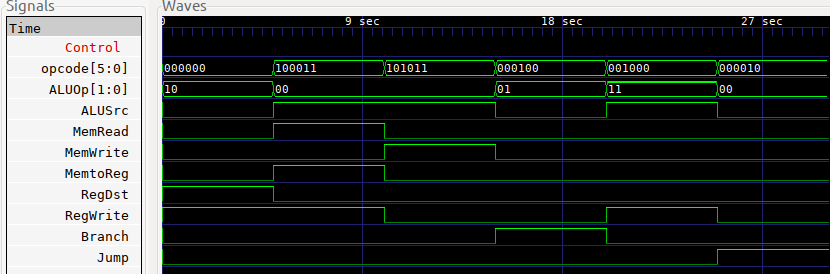
\includegraphics[width=\columnwidth]{Lab-Tex/Lab5-images/t1.png}
    \captionof{figure}{Wave output of control unit test bench}
    \medskip
\endgroup


\subsection{ALUControl Unit Test Bench}

To test the ALUControl, the ALUOp and funct from Table 3 in the lab assignment were cycled through once. Once again, the outputs match that of the given table.

\begingroup
    \centering
    \medskip
    %width=\columnwidth
    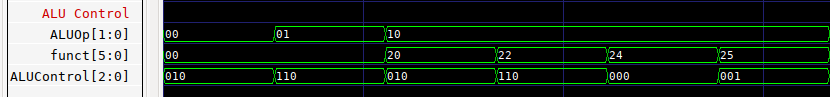
\includegraphics[width=\columnwidth]{Lab-Tex/Lab5-images/t2.png}
    \captionof{figure}{Wave output of control unit test bench}
    \medskip
\endgroup

\subsection{Sample.s Program}

The screenshot below shows the program counter along with the instructions being executed in that cycle. We see that after the PC arrives to address 36, it returns up to address 28. This is representative of the branch condition being unfulfilled and the jump leading the PC back up to address 28. \\

\begingroup
    \centering
    \medskip
    %width=\columnwidth
    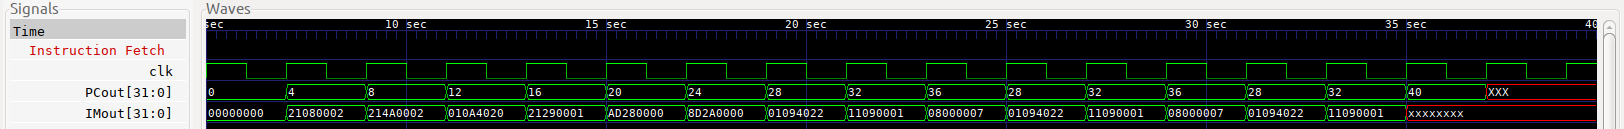
\includegraphics[width=\columnwidth]{Lab-Tex/Lab5-images/p1.png}
    \captionof{figure}{Wave output of program counter and instruction memory output}
    \medskip
\endgroup

However, in the second-to-last cycle in the image above, we see that the PC branches from 32 to 40, showing that the branch condition was fulfilled and the program execution was completed. \\

Next, we take a look at the registers and the values they contain. We see that the registers being accessed correspond with those requested by the instruction. For example, the first instruction requires register \cc{\$t0}, or 8, for read and write. The initial value stored is \cc{0}, but we see the \cc{RFWriteData} signal carrying \cc{2} to write into register \cc{\$t0}. \\

\begingroup
    \centering
    \medskip
    %width=\columnwidth
    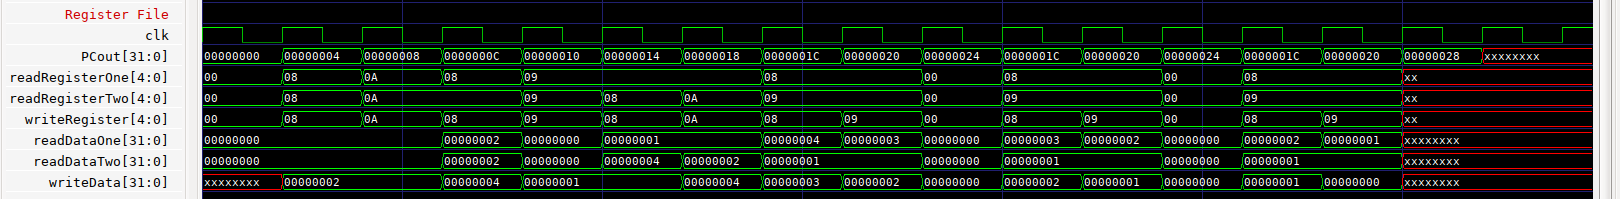
\includegraphics[width=\columnwidth]{Lab-Tex/Lab5-images/p2.png}
    \captionof{figure}{Wave output of registers and register values}
    \medskip
\endgroup
\\

Then, we consider the output of the control module, which receives the opcode as an input. \\

Going in order, we see that the \cc{RegWrite} signal is enabled throughout the program, except for the instructions at addresses \cc{20, 32, 36}, the \cc{sw, beq, and j} instructions, respectively. \\

We also see that \cc{RegDst} and \cc{ALUSrc} enable on instructions where an alternate source for a signal is required. \\ 

The \cc{memRead} signal enables only once for the instruction at address \cc{24}, while \cc{memWrite}  and \cc{MemtoReg} signal enable only once for the instruction at address \cc{20}. These correspond the the \cc{lw} and \cc{sw} instructions, respectively.\\

The \cc{BranchCtrl} signal is enabled at every branch instruction, but we see that the \cc{Branch} signal is enabled only once in the second-to-last cycle.\\

On the other hand, the jump signal is enabled at every jump instruction, as it is an unconditional jump.\\

\begingroup
    \centering
    \medskip
    %width=\columnwidth
    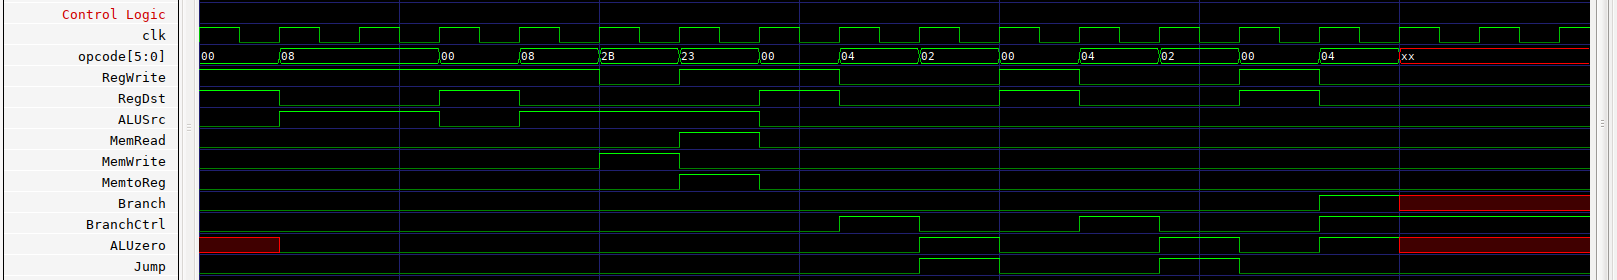
\includegraphics[width=\columnwidth]{Lab-Tex/Lab5-images/p3.png}
    \captionof{figure}{Wave output of the control unit}
    \medskip
\endgroup
\\

The ALU is controlled with the \cc{ALUControl} module, which receives input from the funct slice of the instruction and the ALUOp from the control logic. \\

Here we see that the \cc{ALUControl} unit is able to send the signal for the correct arithmetic operation despite the variety of \cc{funct} and \cc{ALUOp} codes. The first 6 instructions, despite being quite different, all require the \cc{ALU} to carry out addition, which is what \cc{010} implies. \\

\begingroup
    \centering
    \medskip
    %width=\columnwidth
    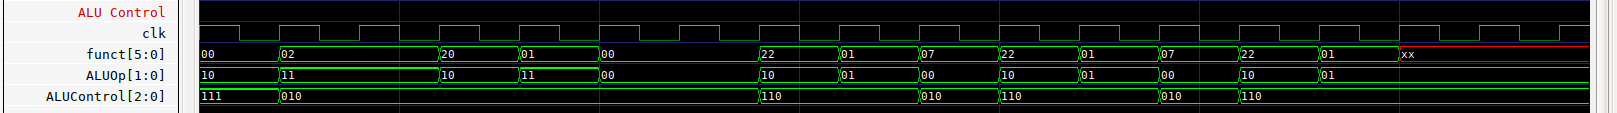
\includegraphics[width=\columnwidth]{Lab-Tex/Lab5-images/p4.png}
    \captionof{figure}{Wave output of the ALU control unit}
    \medskip
\endgroup
\\

We also take a look at the ALU to see the outputs of the arithmetic. Looking at the instructions corresponding to \cc{PCOut} at \cc{28} and \cc{32}, we see the \cc{110 funct} code. Here, the the instruction at \cc{28} is the \cc{sub} instruction carrying out a subtraction to update the value of register \cc{\$t0}. The next instruction is the \cc{beq} carrying out a check. We see that the output of the \cc{sub} instruction becomes the input of the next \cc{ALU} operation. We also see that the \cc{zero} flag is raised on the unconditional jump instructions and when \cc{beq} is executed. \\

\begingroup
    \centering
    \medskip
    %width=\columnwidth
    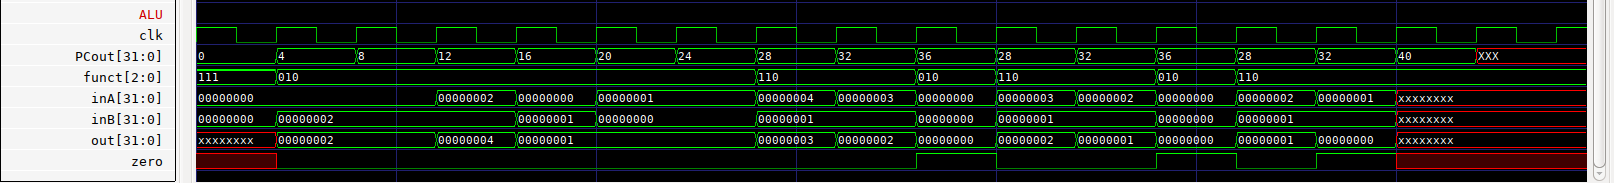
\includegraphics[width=\columnwidth]{Lab-Tex/Lab5-images/p5.png}
    \captionof{figure}{Wave output of the ALU}
    \medskip
\endgroup
\\

Finally, we look at the register values. Register\cc{\$t1} remains the value \cc{1} it was assigned using the \cc{addi} instruction. Register\cc{\$t2} changes from the \cc{lw} instruction, while the data memory updates due to the \cc{sw} instruction.  Register\cc{\$t0} decrements from \cc{4} to \cc{1}, when it is then equal to \cc{\$t1} and the branch executes. \\

\begingroup
    \centering
    \medskip
    %width=\columnwidth
    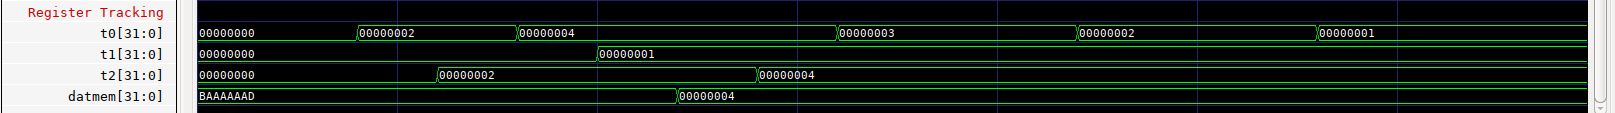
\includegraphics[width=\columnwidth]{Lab-Tex/Lab5-images/p6.png}
    \captionof{figure}{Wave output of registers and data memory}
    \medskip
\endgroup
\\

\section{Conclusion}

This single-cycle implementation of the CPU is now capable of carrying out branch and jump instructions as well as selecting datapaths without hard-coded control logic. 



%%%%%%%%%%%%%%%%%%%%%%%%%%5
% BIBLIOGRAFIA 
% Estilo de bibliografia ABNT. Se não tiver instalado, mude para plain ou ieeetr

%\bibliographystyle{plain} % Inclua isso se não tiver ABNTEX instalado
% \begin{thebibliography}{refs}
% \bibitem{}
\printbibliography
% \end{thebibliography}
\end{document}